% Final presentation – Beamer version of docs/presentation/slides_outline.md (14 slides, ~15 min)
% Build:  latexmk -pdf slides.tex   (run inside docs/latex/)
\documentclass[aspectratio=169,11pt]{beamer}

\usetheme[progressbar=frametitle, numbering=fraction]{metropolis}
\usepackage[T1,T5]{fontenc}
\usepackage[utf8]{inputenc}
\usepackage{lmodern}
\usepackage[vietnamese,main=english]{babel}
\usepackage{amsmath}
\usepackage{booktabs}
\usepackage{array}
\usepackage{graphicx}
\usepackage{listings}
\usepackage{tikz}
\usetikzlibrary{arrows.meta,positioning}

\graphicspath{{../figures/}{figures/}}

\tikzset{st/.style={draw, rounded corners=3pt, align=center, text width=2.15cm, minimum height=1.5cm,
                    font=\footnotesize, fill=#1}, st/.default=accent!12}

\definecolor{accent}{HTML}{1F5FA8}
\definecolor{warn}{HTML}{D2691E}
\definecolor{codebg}{HTML}{F6F6F4}
\setbeamercolor{alerted text}{fg=warn}
\setbeamercolor{progress bar}{fg=accent, bg=accent!15}
\setbeamercolor{frametitle}{bg=accent!85!black}
\setbeamercolor{title separator}{fg=accent}

\lstset{basicstyle=\ttfamily\scriptsize, backgroundcolor=\color{codebg}, frame=single,
  rulecolor=\color{gray!40}, columns=fullflexible, keepspaces=true, language=C++,
  keywordstyle=\color{accent}\bfseries, commentstyle=\color{gray}\itshape,
  morekeywords={pragma,omp,parallel,schedule,runtime}}

\newcommand{\x}{\ensuremath{\times}}
\newcommand{\us}{\,\textmu s}
\newcommand{\bignum}[1]{{\usebeamerfont{title}\color{accent}\textbf{#1}}}

\title{Parallel Seam Carving with OpenMP}
\subtitle{Content-aware image resizing on a multicore CPU}
\author{Đỗ Tùng Dương, Hoàng Trọng Đại, Lê Quang Huy}
\institute{MAT3148 -- Tính Toán Song Song \\ VNU University of Science (VNU-HUS)}
\date{26/11/2026}

\begin{document}

% 1 -------------------------------------------------------------------------
\begin{frame}[plain]
  \begin{columns}[c]
    \begin{column}{0.55\textwidth}
      {\usebeamerfont{title}\usebeamercolor[fg]{title}\insertshorttitle\par}
      \vspace{4pt}
      {\usebeamerfont{subtitle}\insertsubtitle\par}
      \vspace{4pt}{\color{accent}\rule{\linewidth}{0.6pt}}\vspace{6pt}
      \small\insertauthor\par\insertinstitute\par\insertdate
    \end{column}
    \begin{column}{0.4\textwidth}\centering
      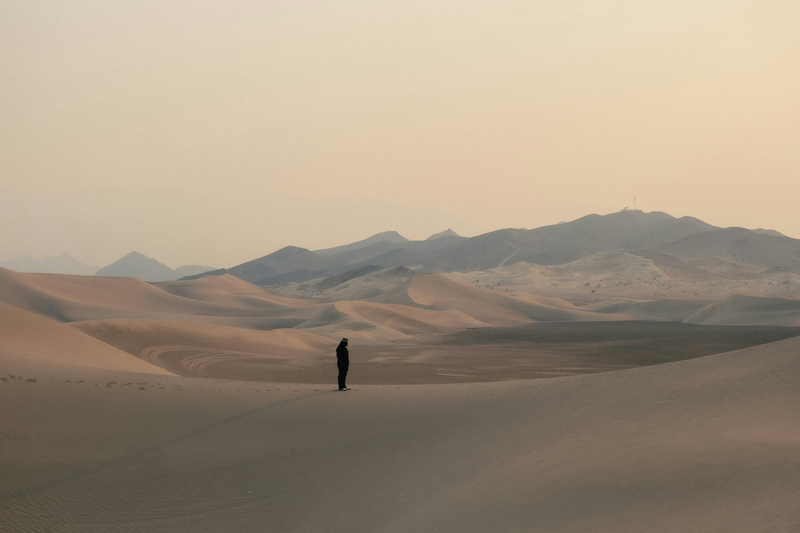
\includegraphics[height=2.6cm]{original.png}\\[2pt]
      \tiny $800\times533$ \quad$\downarrow$\quad seam carved to $560\times533$\\[3pt]
      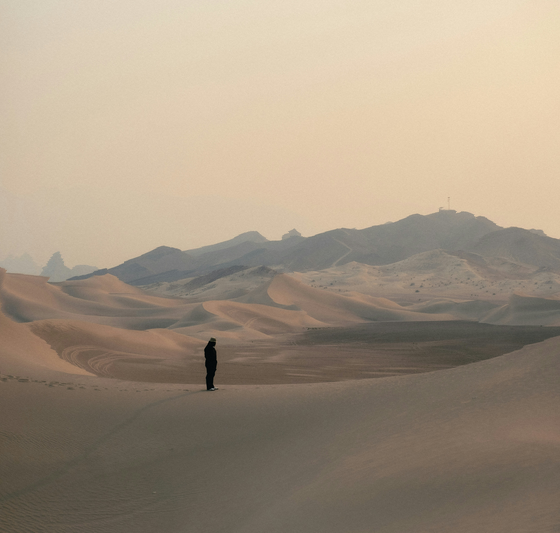
\includegraphics[height=2.6cm]{carved.png}
    \end{column}
  \end{columns}
\end{frame}

% 2 -------------------------------------------------------------------------
\begin{frame}{What is seam carving?}
  \begin{itemize}
    \item Shrink an image by removing the \alert{least important connected path of pixels} (a seam),
          one at a time.
    \item Keeps the important content; scaling distorts it, cropping cuts it off.
  \end{itemize}
  \vspace{4pt}
  \centering
  \begin{tabular}{@{}cccc@{}}
    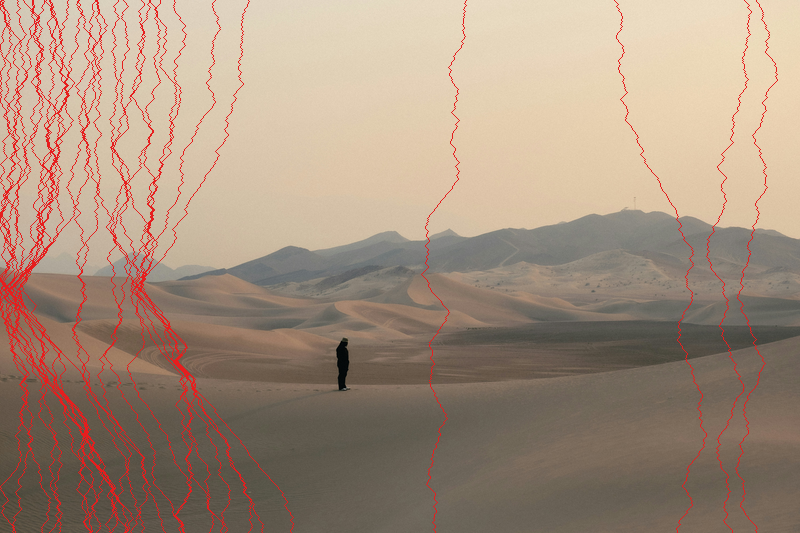
\includegraphics[height=2.8cm]{seams.png} &
    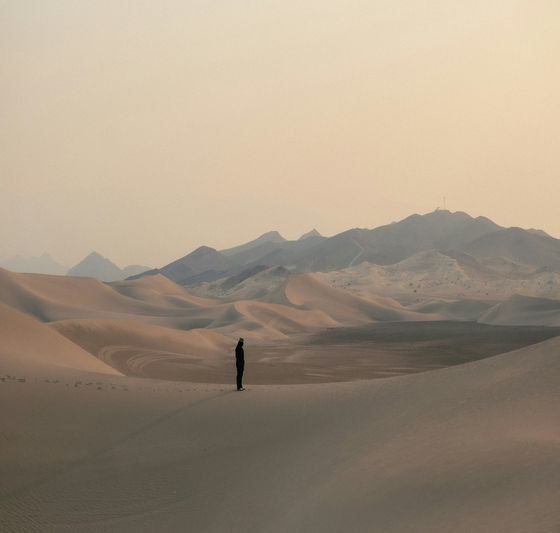
\includegraphics[height=2.8cm]{scaled.png} &
    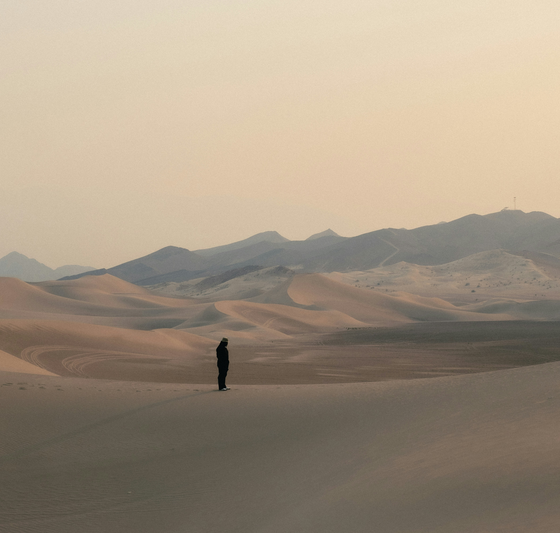
\includegraphics[height=2.8cm]{cropped.png} &
    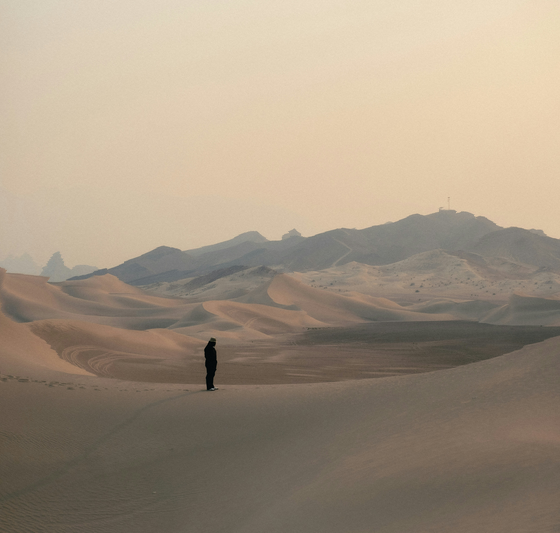
\includegraphics[height=2.8cm]{carved.png} \\
    \scriptsize first 30 seams & \scriptsize scaled & \scriptsize cropped & \scriptsize \textbf{seam carved}
  \end{tabular}\\[4pt]
  \raggedleft\tiny Avidan \& Shamir, SIGGRAPH 2007. Photo: Unsplash (see \texttt{images/SOURCES.md}).
\end{frame}

% 3 -------------------------------------------------------------------------
\begin{frame}{The algorithm}
  \begin{columns}[T]
    \begin{column}{0.5\textwidth}
      \small
      \begin{enumerate}
        \item Energy\quad $e(x,y)=|\partial I/\partial x|+|\partial I/\partial y|$
        \item DP\quad $M(x,y)=e(x,y)+\min\bigl(M(x{-}1,y{-}1),$\\
              \hspace*{5.2em}$M(x,y{-}1),M(x{+}1,y{-}1)\bigr)$
        \item Minimum of the last row
        \item Backtrack to row 0
        \item Remove the seam, shift pixels left
      \end{enumerate}
      \vspace{6pt}
      Repeat $k$ times $\Rightarrow$ cost $\Theta(k\cdot W\cdot H)$.\\[4pt]
      \small Tie rule: smallest column wins.
    \end{column}
    \begin{column}{0.48\textwidth}
      \centering\footnotesize\setlength{\tabcolsep}{4pt}
      Energy $e$ \hspace{5.5em} Cumulative $M$\\[2pt]
      \begin{tabular}{rrrr}\toprule 50&\textbf{\color{warn}30}&50&30\\ 60&60&\textbf{\color{warn}30}&50\\
        70&\textbf{\color{warn}50}&20&50\\ \textbf{\color{warn}30}&70&80&90\\\bottomrule\end{tabular}\quad
      \begin{tabular}{rrrr}\toprule 50&\textbf{\color{warn}30}&50&30\\ 90&90&\textbf{\color{warn}60}&80\\
        160&\textbf{\color{warn}110}&80&110\\ \textbf{\color{warn}140}&150&160&170\\\bottomrule\end{tabular}\\[6pt]
      \footnotesize Seam $s=[1,2,1,0]$, cost $30+30+50+30=140$\\
      (row 0: tie between $x=1$ and $x=3$ $\to$ $x=1$)
    \end{column}
  \end{columns}
\end{frame}

% 4 -------------------------------------------------------------------------
\begin{frame}{Where is the parallelism?}
  Seams are \alert{sequential}: seam $i+1$ is defined on the image left by seam $i$.\\
  All parallelism is \emph{inside} one seam:
  \vspace{10pt}

  \centering
  \begin{tikzpicture}[>=Stealth, node distance=0.3cm]
    \node[st] (E) {\textbf{1 Energy}\\rows independent\\\texttt{parallel for}};
    \node[st=warn!20, right=of E] (D) {\textbf{2 DP}\\row $y$ needs $y-1$\\\alert{1 barrier per row}};
    \node[st, right=of D] (M) {\textbf{3 Minimum}\\reduction};
    \node[st=gray!15, right=of M] (B) {\textbf{4 Backtrack}\\dependent chain\\sequential};
    \node[st, right=of B] (R) {\textbf{5 Removal}\\rows independent\\\texttt{parallel for}};
    \draw[->] (E) -- (D); \draw[->] (D) -- (M); \draw[->] (M) -- (B); \draw[->] (B) -- (R);
    \draw[->] (R.south) -- ++(0,-0.45) -| node[pos=0.25, below, font=\footnotesize]{next seam ($k$ times)} (E.south);
  \end{tikzpicture}
  \vspace{8pt}

  \raggedright
  $1920\times1080$, 384 seams $\Rightarrow$ \alert{414\,336 DP barriers}, each protecting $\approx2$\us{} of work.
\end{frame}

% 5 -------------------------------------------------------------------------
\begin{frame}{Three versions, one answer}
  \begin{columns}[T]
    \begin{column}{0.44\textwidth}
      \begin{itemize}
        \item \textbf{Sequential} -- baseline, no OpenMP
        \item \textbf{M2 OpenMP} -- each stage parallelized directly
        \item \textbf{M5 optimized} -- less work, less memory, fewer barriers
      \end{itemize}
      \vspace{8pt}
      Integer arithmetic + fixed tie rule\\
      $\Rightarrow$ \alert{bit-identical output} for any thread count and schedule.
    \end{column}
    \begin{column}{0.54\textwidth}
      \centering\small
      \begin{tabular}{@{}r>{\raggedright\arraybackslash}p{3.3cm}@{}}
        \bignum{$\approx$237\,000} & test checks, 0 failed \\[4pt]
        \bignum{18 / 18} & mutants detected \\[4pt]
        \bignum{1905 / 1905} & benchmark outputs identical \\[4pt]
        \bignum{0} & sanitizer reports (ASan, UBSan, TSan) \\
      \end{tabular}
    \end{column}
  \end{columns}
\end{frame}

% 6 -------------------------------------------------------------------------
\begin{frame}[fragile]{Basic OpenMP implementation (M2)}
  \lstset{basicstyle=\ttfamily\fontsize{6.5}{7.5}\selectfont}
  \begin{columns}[T]
    \begin{column}{0.45\textwidth}
      \footnotesize Energy / removal: rows independent
\begin{lstlisting}
#pragma omp parallel for schedule(runtime)
for (int y = 0; y < height; ++y)
    removeRow(image, gray, width, seam[y], y);
\end{lstlisting}
      \footnotesize DP variant A: one parallel loop per row
\begin{lstlisting}
for (int y = 1; y < height; ++y) {
    #pragma omp parallel for schedule(runtime)
    for (int x = 0; x < width; ++x)
        m[x] = dpCell(prev, e, width, x);
}   // implicit barrier = row y finished
\end{lstlisting}
    \end{column}
    \begin{column}{0.53\textwidth}
      \scriptsize
      \begin{tabular}{@{}>{\raggedright\arraybackslash}p{1.6cm}>{\raggedright\arraybackslash}p{2.7cm}>{\raggedright\arraybackslash}p{2.6cm}@{}}
        \toprule
        Where & Possible race & Prevented by \\
        \midrule
        DP row $y$ & reading row $y-1$ before it is written & barrier after every row \\
        Minimum & two threads, same slot & one slot per thread \\
        Energy, removal & none: own row only & -- \\
        Next stage & reads unfinished data & barrier at end of region \\
        \bottomrule
      \end{tabular}\\[6pt]
      Positive control: remove the DP barrier $\to$ 75 failed checks, TSan reports 83 races.
    \end{column}
  \end{columns}
\end{frame}

% 7 -------------------------------------------------------------------------
\begin{frame}{Result 1: the parallel DP is \emph{slower} than sequential}
  \begin{columns}[c]
    \begin{column}{0.4\textwidth}
      Platform A: i7-1065G7, Windows, GCC/libgomp
      \vspace{8pt}
      \begin{itemize}
        \item All four stages parallel: \alert{0.01--0.68\x}
        \item More threads $\Rightarrow$ \alert{slower}
        \item DP kept sequential: \textbf{1.40--1.79\x}\\(images $\ge 1920\times1080$)
      \end{itemize}
    \end{column}
    \begin{column}{0.58\textwidth}
      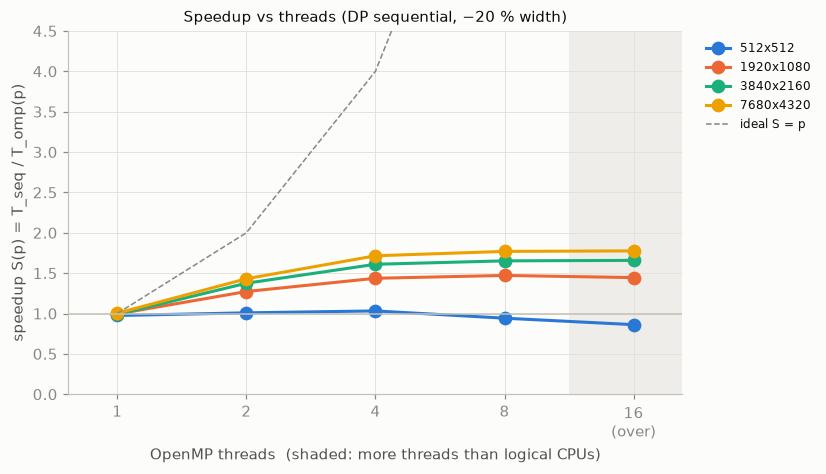
\includegraphics[width=\linewidth]{speedup_vs_threads_main_nodp.png}\\
      \tiny M2 with DP sequential, Platform A
    \end{column}
  \end{columns}
\end{frame}

% 8 -------------------------------------------------------------------------
\begin{frame}{Why? Synchronization cost}
  \begin{columns}[c]
    \begin{column}{0.47\textwidth}
      \begin{itemize}
        \item One DP row: \textbf{1.84\us} of work
        \item One barrier on Windows: \alert{22--167\us}
        \item $414\,336 \times 45\us \approx 18.8$\,s\\$\approx$ measured 19.6\,s \emph{(calculation)}
        \item Same code on Linux: barrier $\approx1$\us{} $\to$ parallel DP no longer slower
        \item Amdahl, DP sequential ($f\approx0.4$): max $\approx$ \textbf{2.5\x}
      \end{itemize}
    \end{column}
    \begin{column}{0.51\textwidth}
      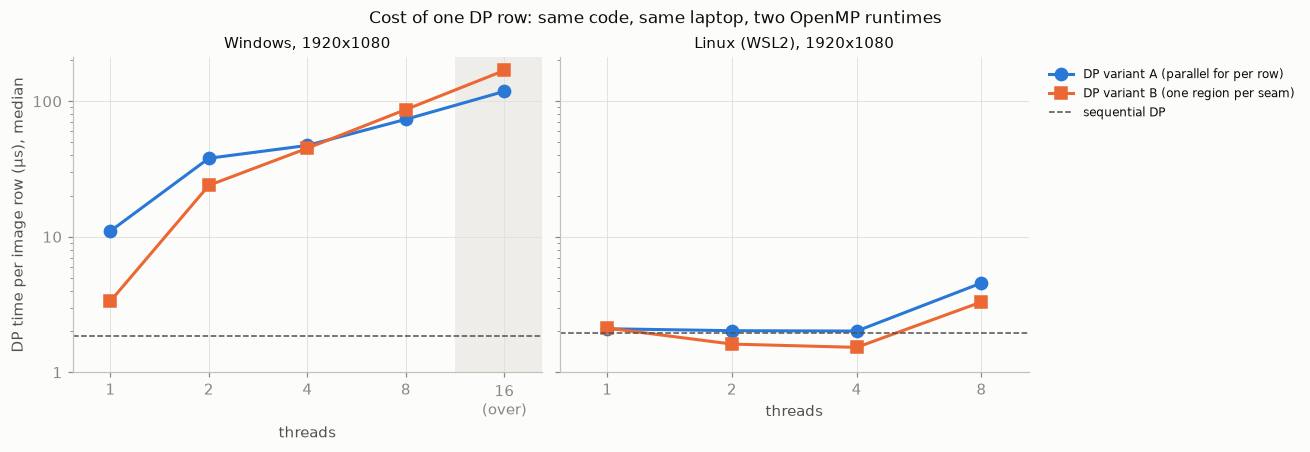
\includegraphics[width=\linewidth]{dp_time_per_row.png}\\
      \tiny DP time per image row, Platform A
    \end{column}
  \end{columns}
\end{frame}

% 9 -------------------------------------------------------------------------
\begin{frame}{Optimizations (M5)}
  \begin{columns}[c]
    \begin{column}{0.45\textwidth}
      \small
      \begin{description}[O2]
        \item[O2] SIMD kernels: branch-free interior loops
        \item[O1] incremental energy: only 2 values per row change
        \item[O5] compact memory: 16-bit energy, 1-byte directions
        \item[O3] blocked DP: \alert{1 barrier per 64 rows}, halo cells
      \end{description}
      \vspace{4pt}
      Each one switchable and measured separately.
    \end{column}
    \begin{column}{0.53\textwidth}
      \centering
      \begin{tikzpicture}[x=0.3cm,y=0.42cm]
        \def\a{8}\def\b{14}\def\K{4}
        \foreach \j in {0,...,3} {
          \pgfmathtruncatemacro{\h}{\K-1-\j}
          \pgfmathtruncatemacro{\lo}{\a-\h}
          \pgfmathtruncatemacro{\hi}{\b+\h}
          \fill[warn!30] (\lo,-\j) rectangle (\a,-\j-1);
          \fill[warn!30] (\b,-\j) rectangle (\hi,-\j-1);
          \fill[accent!40] (\a,-\j) rectangle (\b,-\j-1);
        }
        \draw[gray!60, step=1] (3,0) grid (19,-4);
        \fill[gray!25] (3,1.2) rectangle (19,0.2);
        \draw[gray!60] (3,1.2) grid (19,0.2);
        \node[font=\tiny, above] at (11,1.2) {last row of previous block (shared)};
        \draw[very thick, warn] (3,-4.35) -- (19,-4.35);
        \node[font=\tiny, below, text=warn] at (11,-4.4) {\textbf{barrier} -- one per block};
        \node[font=\tiny, anchor=west] at (3,-6) {\textcolor{accent!70}{\rule{5pt}{5pt}} own columns of one thread};
        \node[font=\tiny, anchor=west] at (3,-6.9) {\textcolor{warn!70}{\rule{5pt}{5pt}} halo: computed redundantly, private};
      \end{tikzpicture}\\[2pt]
      \tiny $K=4$ shown; halo shrinks one column per side per row
    \end{column}
  \end{columns}
\end{frame}

% 10 ------------------------------------------------------------------------
\begin{frame}{Step-by-step effect ($1920\times1080$, 8 threads)}
  \begin{columns}[c]
    \begin{column}{0.42\textwidth}
      \small
      \begin{tabular}{@{}lrr@{}}
        \toprule
        Step & time (s) & speedup \\
        \midrule
        sequential & 2.160 & 1.00 \\
        M2, DP sequential & 1.378 & 1.57 \\
        M5, all off & 1.435 & 1.51 \\
        + SIMD (O2) & 0.944 & 2.29 \\
        + incremental (O1) & 0.850 & 2.54 \\
        + compact (O5) & 0.764 & 2.83 \\
        + blocked DP (O3) & \textbf{0.479} & \textbf{4.51} \\
        \bottomrule
      \end{tabular}\\[2pt]
      \tiny Platform B, median of 5 runs
    \end{column}
    \begin{column}{0.56\textwidth}
      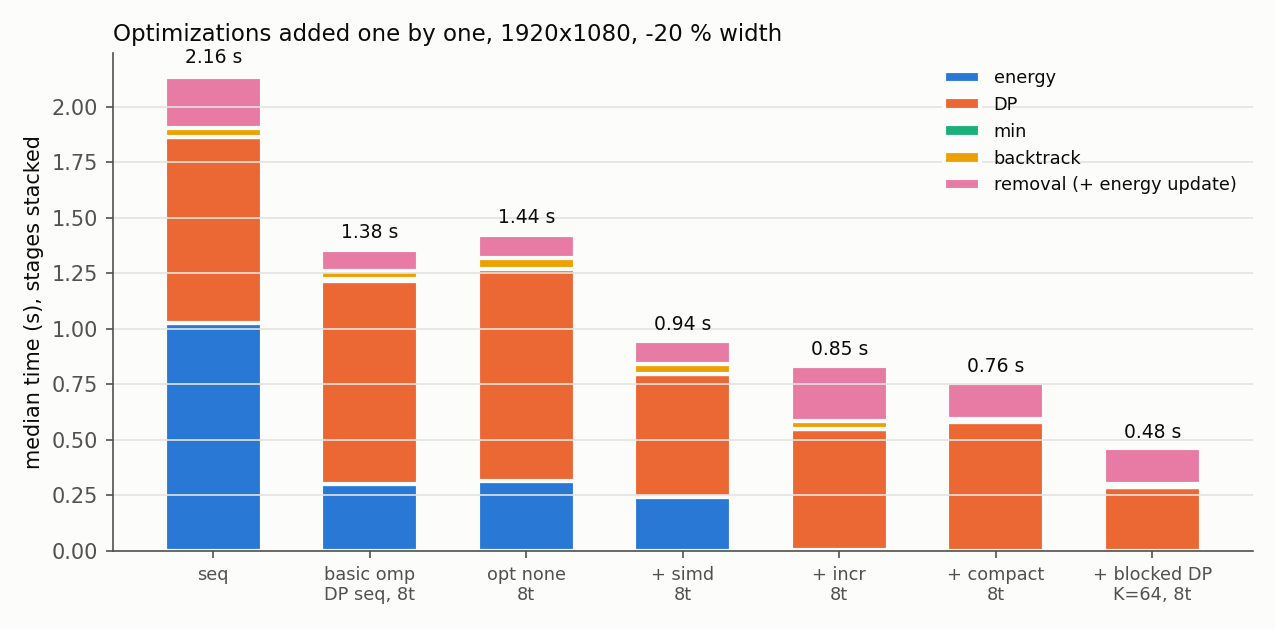
\includegraphics[width=\linewidth]{m5_ablation_1920x1080.png}
    \end{column}
  \end{columns}
\end{frame}

% 11 ------------------------------------------------------------------------
\begin{frame}{Key insight: memory, not threads}
  \begin{columns}[c]
    \begin{column}{0.44\textwidth}
      \begin{itemize}
        \item Blocked DP \emph{alone}: 0.547 $\to$ 0.512\,s
        \item Blocked DP \emph{with compact memory}: 0.580 $\to$ \alert{0.287\,s}
        \item DP working set: 16.6\,MB ($>$ 8\,MB L3) $\to$ 6.2\,MB ($<$ L3) \emph{(calculation)}
      \end{itemize}
      \vspace{6pt}
      Fewer barriers help only once the data fits in the cache.
    \end{column}
    \begin{column}{0.54\textwidth}
      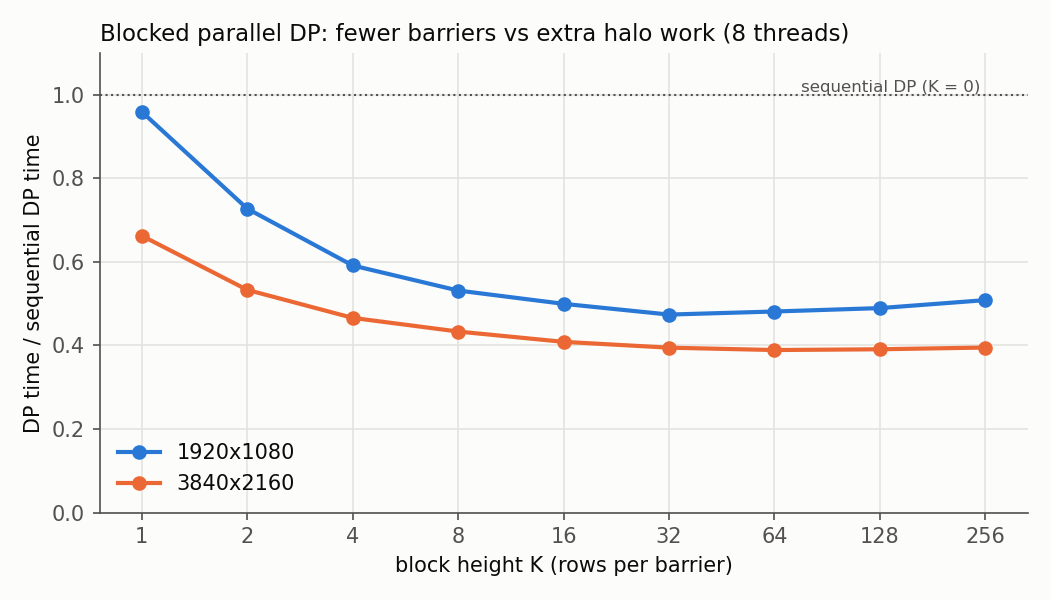
\includegraphics[width=\linewidth]{m5_dp_block.png}\\
      \tiny DP time vs.\ block height $K$, 8 threads; $K=64$ default
    \end{column}
  \end{columns}
\end{frame}

% 12 ------------------------------------------------------------------------
\begin{frame}{Final speedup}
  \begin{columns}[c]
    \begin{column}{0.36\textwidth}
      \bignum{4.4--4.8\x}\\ \small over sequential, 8 threads\\(Ryzen 7 4800H, Linux container)
    \end{column}
    \begin{column}{0.6\textwidth}
      \begin{itemize}\small
        \item M2 on same machine: 1.5--1.6\x
        \item 2.4\x{} already with \emph{one} thread (less work)
        \item 16 threads slower than 8 (SMT)
      \end{itemize}
    \end{column}
  \end{columns}
  \vspace{4pt}
  \centering
  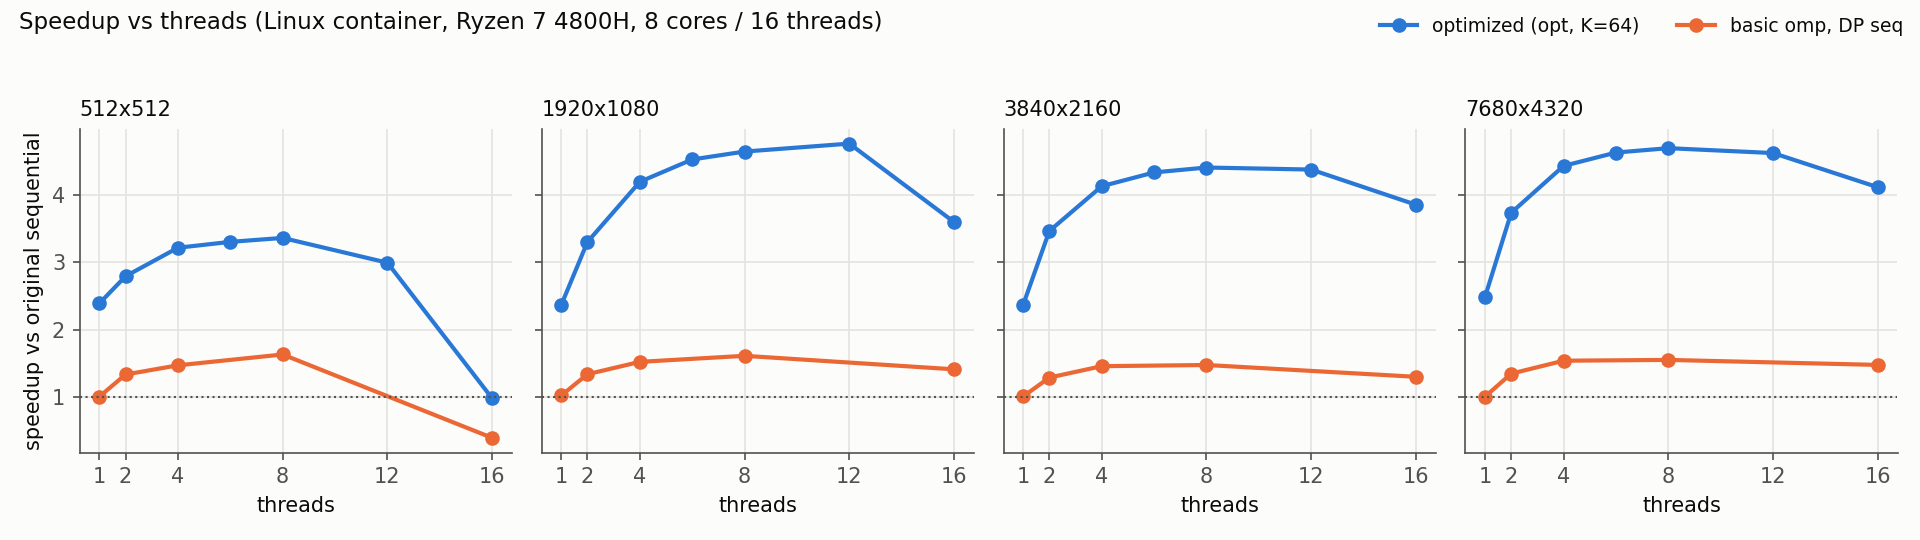
\includegraphics[width=\textwidth]{m5_speedup_threads.png}\\
  \tiny blue: optimized (M5), orange: best M2 configuration, Platform B
\end{frame}

% 13 ------------------------------------------------------------------------
\begin{frame}{Limitations and what we learned}
  \begin{columns}[T]
    \begin{column}{0.48\textwidth}
      \textbf{Limitations}
      \begin{itemize}\small
        \item Seam removal $\approx18$\,GB/s vs.\ 19.6\,GB/s copy bandwidth $\to$ \alert{memory-bound}
        \item Two machines / OSes; M5 in a Linux container on WSL2
        \item Memory traffic estimated, no hardware counters
        \item Only basic $e_1$ energy, no enlarging
      \end{itemize}
    \end{column}
    \begin{column}{0.48\textwidth}
      \textbf{Lessons}
      \begin{itemize}\small
        \item Measure before optimizing
        \item Synchronization granularity decides fine-grained parallelism
        \item Data size matters as much as thread count
        \item Bit-exact testing makes optimization safe
      \end{itemize}
    \end{column}
  \end{columns}
\end{frame}

% 14 ------------------------------------------------------------------------
\begin{frame}{Conclusion}
  \begin{itemize}
    \item Correct parallel seam carving with \textbf{bit-identical} output
    \item \alert{4.4--4.8\x} speedup, explained stage by stage
    \item Barrier cost and memory traffic, not core count, set the limit
  \end{itemize}
  \vspace{6pt}
  \textbf{Future work:} avoid physical pixel shifts, forward energy, LLVM libomp on Windows, GPU.
  \vspace{18pt}

  \centering{\Large\color{accent}\textbf{Questions?}}
\end{frame}

\end{document}
